

\tikzset{every picture/.style={line width=0.75pt}} %set default line width to 0.75pt        

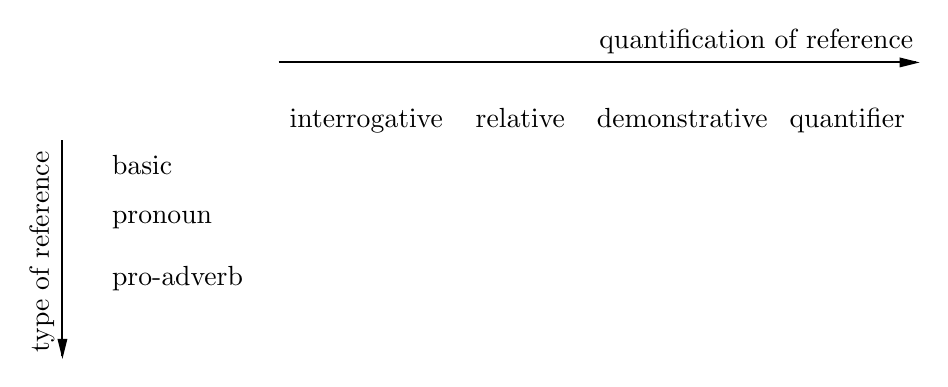
\begin{tikzpicture}[x=0.75pt,y=0.75pt,yscale=-0.8,xscale=0.8]
%uncomment if require: \path (0,359); %set diagram left start at 0, and has height of 359

%Straight Lines [id:da31021882936115297] 
\draw    (245.21,31) -- (629.21,31) ;
\draw [shift={(631.21,31)}, rotate = 180] [fill={rgb, 255:red, 0; green, 0; blue, 0 }  ][line width=0.08]  [draw opacity=0] (12,-3) -- (0,0) -- (12,3) -- cycle    ;
%Straight Lines [id:da4548639136296362] 
\draw    (115,78) -- (115,207.5) ;
\draw [shift={(115,209.5)}, rotate = 270] [fill={rgb, 255:red, 0; green, 0; blue, 0 }  ][line width=0.08]  [draw opacity=0] (12,-3) -- (0,0) -- (12,3) -- cycle    ;

% Text Node
\draw (629.21,28) node [anchor=south east] [inner sep=0.75pt]   [align=left] {quantification of reference};
% Text Node
\draw (112,207.5) node [anchor=south west] [inner sep=0.75pt]  [rotate=-270] [align=left] {type of reference};
% Text Node
\draw (250,57) node [anchor=north west][inner sep=0.75pt]   [align=left] {interrogative};
% Text Node
\draw (362,57) node [anchor=north west][inner sep=0.75pt]   [align=left] {relative};
% Text Node
\draw (435,57) node [anchor=north west][inner sep=0.75pt]   [align=left] {demonstrative};
% Text Node
\draw (551,57) node [anchor=north west][inner sep=0.75pt]   [align=left] {quantifier};
% Text Node
\draw (143,85) node [anchor=north west][inner sep=0.75pt]   [align=left] {basic};
% Text Node
\draw (143,119) node [anchor=north west][inner sep=0.75pt]   [align=left] {pronoun};
% Text Node
\draw (143,152) node [anchor=north west][inner sep=0.75pt]   [align=left] {pro-adverb};


\end{tikzpicture}
